\chapter{Introduction}
{\color{gray}
 \begin{fquote}[Eduardo Galeano]  Disasters are called natural, as if nature were the executioner and not the victim. \end{fquote} }


Biodiversity, the term used to describe the wide variety of species on Earth, is declining at enormous rates due to human-induced environmental changes. The last time that Earth experienced such high rates of biodiversity loss in a relatively short time was at the end of the Cretaceous period, 65 millon years ago, then most dinosaurs went extinct \cite{wake2008we}. Biodiversity loss, in turn, compromises ecosystem stability and productivity, which negatively impacts the ecosystem services on which human communities depend \cite{tilman2006biodiversity}. \\


%\vspace*{2cm}


%Phylogenetic... blabla... Heal stuff... \\

To conserve biodiversity, we must understand the mechanisms how it comes about and how it is maintained, in assemblages of species, so-called ecological communities. Novel genomic tools make it possible only now to measure and model species in great detail. In the last decade sophisticated methods have been developed that primarily aimed at inferring the evolutionary relatedness of the species (the phylogenetic tree) from DNA sequence data on the basis of models of species diversification. On figure \ref{avian} we can see the phylogenetic tree of the most complete analysis of avian species \cite{jetz2012global}.\\

About 1.7 million species have been identified and given scientific names, but only about $100,000$ of these are popular enough for taxonomist to know them well. There are estimated to be anywhere from 6 to 15 million species on Earth. Many new species are found each year; for instance, 361 new species (mostly insects) were found in the remote rainforest of Borneo from 1999 to 2004 \cite{chivian2008sustaining}. \\

Mathematical and statistical tools have been crucial to generate an understanding on diversification processes \cite{gillman2009introduction}. However there is still a lot to improve. Most of current models have some major shortcomings: they are either too simplistic, too specific or overly complex increasing the dimensionality of the system enormously.\\
% We will briefly review some of them in the next section. \\

% ... All models are wrong.. blabla ... however we can ... \
 
Novel differential geometric approach to statistical methods have been successful implemented on biological data \cite{augugliaro2013differential}\cite{abegaz2013sparse}, and give us a hope to reduce the inferential and computational complexity of the diversification scenario. In this project, we will consider models that account for local interactions and complex ecology information. \\
 
 
This manuscript has been written to be readable for both mathematicians and biologist, as well as a broader audience. Keeping that in mind, in chapter 2 we discuss an overview of the evolutionary diversification process and the ecological mechanism behind it. In chapter 3 we introduce the statistical modeling of the problem step by step. Finally, last tree chapters comment the knowledge utilization of this project, the timeline, and the bibliography respectively. 

%The notation used for the models is included on the appendix. 
%In next chapter we review the current result on the fild as well as describing the... and the biological research questions we will face ... 

%on chapter 3 we describe the mathematical modeling which is going to be applied on this project... blablabla


%Finally we included on the apendix a glosary and the notation used on this chapter, if there is any doubt about any biological or notational concept do not hesitate to go to the appendix to ... 


 \begin{figure}
\centering
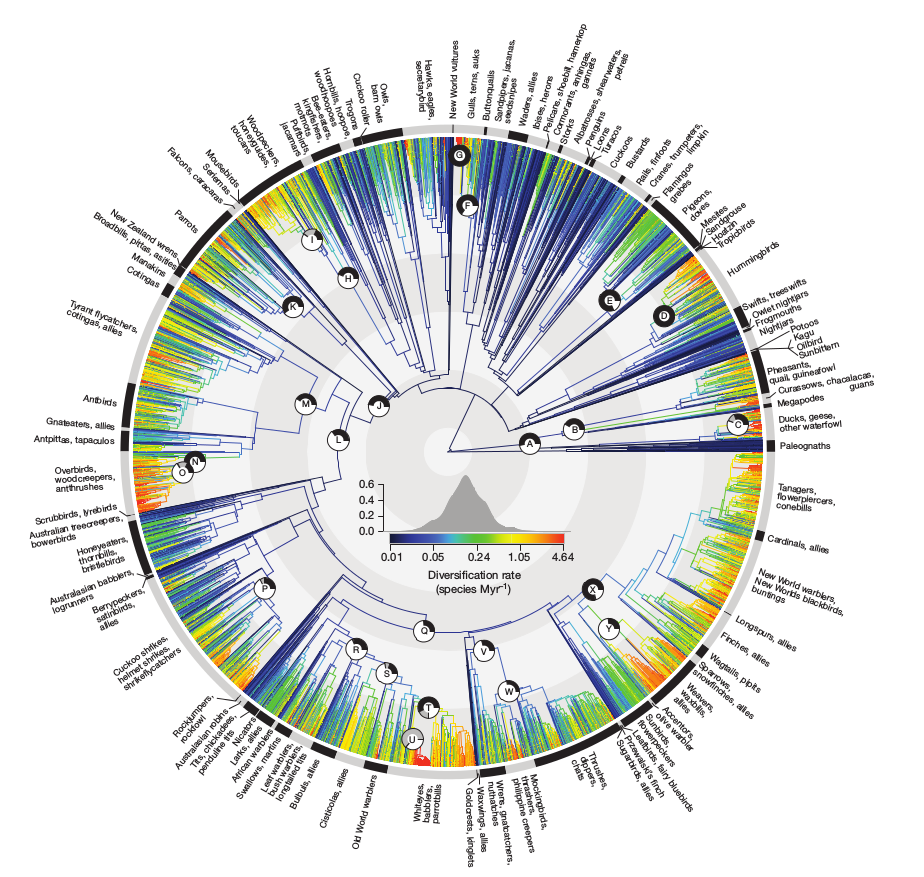
\includegraphics[scale=0.55]{Pictures/birds.png}
\caption{Diversification across the avian tree \cite{jetz2012global}. Public phylogenetic information for avian species is available in this wonderful website http://birdtree.org/.}
\label{avian}
\end{figure}

